\documentclass[a4paper,12pt]{article}
\usepackage[utf8]{inputenc}
\usepackage{amsmath}
\usepackage{graphicx}
\usepackage{hyperref}
\usepackage{tikz}
\usepackage{caption}
\usepackage{xcolor}
\usepackage{listings}
\usepackage{float}
\usepackage{geometry}
\usepackage{times}
\usepackage{titlesec}
\usepackage{booktabs}
\usepackage{multirow}
\usepackage{array}
\usetikzlibrary{positioning, arrows.meta}

% Configuración de página
\geometry{margin=2.5cm}
\setlength{\parskip}{1ex plus 0.5ex minus 0.5ex}

% Colores corporativos
\definecolor{primary}{RGB}{41,128,185}
\definecolor{secondary}{RGB}{52,152,219}
\definecolor{accent}{RGB}{231,76,60}
\definecolor{background}{RGB}{245,245,245}

% Estilos de sección
\titleformat{\section}
{\color{primary}\normalfont\large\bfseries}{\thesection}{1em}{}

% Título
\title{\textbf{Informe del Sistema Distribuido: Arquitectura, Funcionalidades y Procesos}}
\author{Equipo RAFT}
\date{\today}

\begin{document}

\maketitle

\begin{abstract}
Este informe describe el diseño, organización, y ejecución de un sistema distribuido basado en la arquitectura RAFT, que incluye la replicación de datos, manejo de eventos en tiempo real, y el uso de WebSockets para notificaciones. Se detallan las principales funcionalidades del sistema, los procesos involucrados, y las decisiones tomadas para garantizar la consistencia, disponibilidad, y seguridad del sistema. El informe también aborda aspectos relacionados con la tolerancia a fallos y la replicación de datos en un entorno distribuido.
\end{abstract}

\tableofcontents
\newpage

\section{Arquitectura del Sistema}
El sistema distribuido se basa en una arquitectura \textbf{RAFT} que permite la replicación de datos entre varios nodos. La arquitectura se organiza en varios \textit{shards}, cada uno con un líder y seguidores, siguiendo el principio de consenso de RAFT. El objetivo principal de la arquitectura es garantizar la consistencia de los datos en presencia de fallos, mediante la replicación de los logs de eventos.

El sistema también incluye un \textit{layer} de notificaciones en tiempo real basado en el patrón \textbf{Pub/Sub} utilizando WebSockets. Cada usuario está suscrito a un canal de eventos de su interés, lo que permite una comunicación eficiente entre los usuarios del sistema.

\begin{figure}[htbp]
\centering
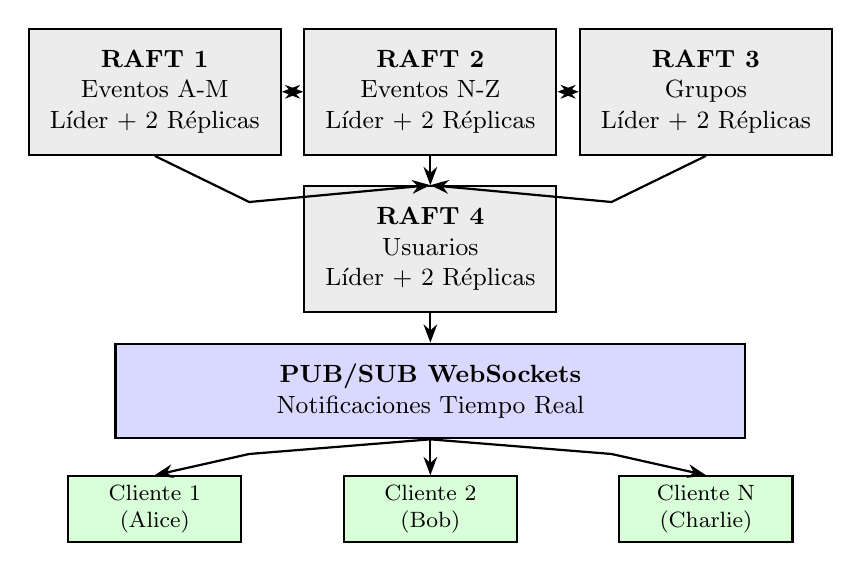
\begin{tikzpicture}[
    raftgroup/.style={rectangle, draw=black, thick, fill=gray!15, minimum width=3.2cm, minimum height=1.6cm, align=center, font=\small},
    pubsub/.style={rectangle, draw=black, thick, fill=blue!15, minimum width=8cm, minimum height=1.2cm, align=center, font=\small},
    client/.style={rectangle, draw=black, thick, fill=green!15, minimum width=2.2cm, minimum height=0.8cm, align=center, font=\footnotesize},
    arrow/.style={-Stealth, thick},
    doublearrow/.style={<->, thick, >=Stealth}
]

% Grupos RAFT superiores
\node[raftgroup] (group1) at (0,0) {\textbf{RAFT 1} \\ Eventos A-M \\ Líder + 2 Réplicas};
\node[raftgroup] (group2) at (3.5,0) {\textbf{RAFT 2} \\ Eventos N-Z \\ Líder + 2 Réplicas};
\node[raftgroup] (group3) at (7,0) {\textbf{RAFT 3} \\ Grupos \\ Líder + 2 Réplicas};

% Conexiones entre grupos RAFT
\draw[doublearrow] (group1.east) -- (group2.west);
\draw[doublearrow] (group2.east) -- (group3.west);

% Grupo RAFT 4 central
\node[raftgroup] (group4) at (3.5,-2) {\textbf{RAFT 4} \\ Usuarios \\ Líder + 2 Réplicas};

% Conexiones a grupo 4
\draw[arrow] (group1.south) -- (1.2,-1.4) -- (group4.north);
\draw[arrow] (group2.south) -- (group4.north);
\draw[arrow] (group3.south) -- (5.8,-1.4) -- (group4.north);

% Layer Pub/Sub
\node[pubsub] (pubsub) at (3.5,-3.8) {\textbf{PUB/SUB WebSockets} \\ Notificaciones Tiempo Real};

% Conexión a Pub/Sub
\draw[arrow] (group4.south) -- (pubsub.north);

% Clientes
\node[client] (client1) at (0,-5.3) {Cliente 1 \\ (Alice)};
\node[client] (client2) at (3.5,-5.3) {Cliente 2 \\ (Bob)};
\node[client] (client3) at (7,-5.3) {Cliente N \\ (Charlie)};

% Conexiones a clientes
\draw[arrow] (pubsub.south) -- (1.2,-4.6) -- (client1.north);
\draw[arrow] (pubsub.south) -- (client2.north);
\draw[arrow] (pubsub.south) -- (5.8,-4.6) -- (client3.north);

\end{tikzpicture}
\caption{Arquitectura del Sistema Distribuido RAFT con WebSockets}
\label{fig:arquitectura}
\end{figure}

\section{Organización del Sistema Distribuido}
El sistema distribuido se organiza en varios componentes clave:

\begin{itemize}
    \item \textbf{Coordinador Inteligente:} Este servicio se encarga de decidir a qué \textit{shard} va cada operación y balancea la carga entre los \textit{shards}.
    \item \textbf{Shards Especializados:} Cada shard gestiona un subconjunto de los datos, como eventos, usuarios, y grupos. Cada shard sigue el protocolo RAFT con un líder y múltiples réplicas.
    \item \textbf{WebSocket Manager:} Administra las conexiones en tiempo real y las notificaciones push.
\end{itemize}

\subsection{Detalle de los Shards}
\begin{table}[htbp]
\centering
\small
\begin{tabular}{p{2.6cm} p{2.2cm} p{2.8cm} p{2.2cm}}
\toprule
\textbf{Shard} & \textbf{Tipo -Datos} & \textbf{Particionamiento} & \textbf{Nodos} \\
\midrule
Shard 1 & Eventos & A-M & 3 (Líder + 2 Réplicas) \\
Shard 2 & Eventos & N-Z & 3 (Líder + 2 Réplicas) \\
Shard 3 & Grupos & Todos & 3 (Líder + 2 Réplicas) \\
Shard 4 & Usuarios & Todos & 3 (Líder + 2 Réplicas) \\
\bottomrule
\end{tabular}
\caption{Distribución de shards en el sistema}
\label{tab:shards}
\end{table}

\section{Roles del Sistema}
Cada nodo en el sistema tiene un rol específico dentro del protocolo RAFT. Los roles incluyen:

\begin{itemize}
    \item \textbf{Líder:} El nodo que coordina la replicación de logs y garantiza la consistencia del sistema.
    \item \textbf{Seguidor:} Nodos que siguen al líder y replican sus logs.
    \item \textbf{Candidato:} Nodos que pueden ser elegidos como líderes si el líder actual falla.
\end{itemize}

\section{Distribución de Servicios en Docker}
El sistema distribuido está implementado en contenedores Docker. Cada grupo de RAFT se ejecuta en contenedores separados, con la comunicación entre los nodos facilitada por Docker Swarm.

\subsection{Redes Docker}
\begin{itemize}
    \item \textbf{raft-network:} Red interna para comunicación entre nodos RAFT
    \item \textbf{api-network:} Red para comunicación frontend-backend
    \item \textbf{public-network:} Red para acceso externo de clientes
\end{itemize}

\section{Procesos del Sistema}
El sistema consta de varios procesos que trabajan en conjunto para garantizar el funcionamiento adecuado:

\begin{itemize}
    \item \textbf{Proceso de Elección de Líder:} Los nodos RAFT eligen un líder para garantizar la consistencia de los datos.
    \item \textbf{Replicación de Logs:} El líder replica sus logs a los nodos seguidores.
    \item \textbf{Notificación en Tiempo Real:} Los clientes se suscriben a canales de eventos y reciben notificaciones a través de WebSockets.
\end{itemize}

\section{Comunicación en el Sistema}
El sistema utiliza varios tipos de comunicación:

\begin{itemize}
    \item \textbf{RPC (Remote Procedure Call):} Usado en el protocolo RAFT para la replicación de logs y la elección de líder.
    \item \textbf{WebSockets:} Usados para la comunicación en tiempo real entre el servidor y los clientes.
    \item \textbf{REST API:} Usada para interactuar con la base de datos del sistema y para la creación y gestión de eventos.
\end{itemize}

\subsection{Flujo de Comunicación}
\begin{enumerate}
    \item Cliente envía solicitud vía WebSocket/REST
    \item Coordinador enruta al shard correspondiente
    \item Líder del shard procesa y replica la operación
    \item Confirmación enviada al cliente
    \item Notificaciones broadcast a clientes interesados
\end{enumerate}

\section{Coordinación del Sistema}
El sistema garantiza que todos los servicios estén sincronizados:

\begin{itemize}
    \item \textbf{Sincronización de Acciones:} A través de RAFT, el líder asegura que las operaciones se apliquen en todos los nodos.
    \item \textbf{Acceso Exclusivo a Recursos:} Se asegura que solo un nodo líder pueda modificar los datos, evitando condiciones de carrera.
\end{itemize}

\section{Tolerancia a Fallos}
El sistema es resiliente a fallos de nodos:

\begin{itemize}
    \item \textbf{Respuesta a Errores:} Si un nodo falla, otro nodo puede ser elegido como líder automáticamente.
    \item \textbf{Nivel de Tolerancia a Fallos:} El sistema puede tolerar la caída de un nodo por cada shard sin interrumpir el servicio.
\end{itemize}

\subsection{Mecanismo de Failover}
\begin{figure}[htbp]
\centering
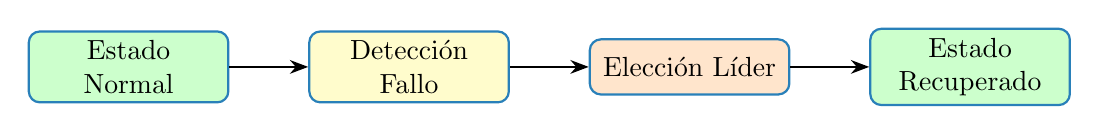
\begin{tikzpicture}[
    state/.style={rectangle, draw=primary, thick, rounded corners, minimum width=2.5cm, minimum height=0.7cm, align=center, text width=2.3cm},
    arrow/.style={-Stealth, thick}
]

\node[state, fill=green!20] (normal) {Estado Normal};
\node[state, fill=yellow!20, right=of normal] (detection) {Detección Fallo};
\node[state, fill=orange!20, right=of detection] (election) {Elección Líder};
\node[state, fill=green!20, right=of election] (recovered) {Estado Recuperado};

\draw[arrow] (normal) -- (detection);
\draw[arrow] (detection) -- (election);
\draw[arrow] (election) -- (recovered);

\end{tikzpicture}
\caption{Proceso de recuperación ante fallos}
\label{fig:failover}
\end{figure}

\section{Seguridad}
La seguridad del sistema se aborda en dos niveles:

\begin{itemize}
    \item \textbf{Seguridad en la Comunicación:} Las comunicaciones entre nodos y clientes están protegidas mediante WebSockets seguros (wss://).
    \item \textbf{Autenticación y Autorización:} Los usuarios deben autenticar su sesión para interactuar con el sistema, y los accesos están restringidos según los roles (líder, miembro, etc.).
\end{itemize}

\subsection{Medidas de Seguridad Implementadas}
\begin{itemize}
    \item Autenticación JWT para usuarios
    \item Encriptación TLS/SSL en todas las comunicaciones
    \item Validación de entrada en todos los endpoints
    \item Logs de auditoría para operaciones críticas
\end{itemize}

\end{document}